\part{Описание текстового синтаксиса с помощью \tool{Grammatic}}

В настоящей главе описан предметно-ориентированный язык \GRM{}, предназначенный для описания текстового синтаксиса и поддерживающий композицию с помощью модулей, шаблонов и аспектов. 

\chapter{Мотивация}

Основным назначением описываемого здесь языка является дополнение существующих инструментов, использующих грамматики, реализацией сложных механизмов композиции. Это достигается за счет предоставления единого формата для представления грамматик, поддерживающего шаблоны и аспекты. Если некоторый инструмент \tool{X} не поддерживает эти механизмы композиции, достаточно разработать генератор, строящий по спецификации на языке \GRM{} спецификацию на входном языке \tool{X}. При таком подходе композицию осуществляет \GRM{}, а инструмент \tool{X} решает ту задачу, для которой он был разработан. Будем называть такой генератор \term{конвертером}. Таким образом, наша цель состоит в том, чтобы обобщенную нотацию для записи контекстно-свободных грамматик, являющуюся надмножеством входных языков существующих инструментов.

Единственной известной нам попыткой разработки обобщенного формата для представления грамматик, полученных из различных источников, является BGF \cite{RecoverJLS}. Этот формат поддерживает все операции EBNF, но никак не обрабатывает аннотации и не поддерживает механизмов композиции.

Реализация \GRM{} представляет собой библиотеку, позволяющую транслировать текстовые описания грамматик во внутреннее объектно-ориентированное представление на основе библиотеки \tool{EMF} \cite{EMF}, к которому имеется открытый программный интерфейс. С использованием этой библиотеки разрабатываются конвертеры, преобразующие спецификации в обобщенной нотации к формату входных данных существующих инструментов.

Основные решения, принятые при проектировании \GRM{}, мотивированы следующими свойствами существующих инструментов.

\paragraph*{Операции расширенной нотации \tool{BNF}.}
В каноническом виде КСГ строятся с помощью двух операций: $\rightarrow$ для формирования продукции и \term{конкатенация} для формирования правой части продукции. В инструментах семейства \tool{Yacc} (например, \cite{YACC}), порождающих восходящие анализаторы, фактически используются только эти две операции, что отвечает содержанию нотации BNF.

Однако при построении нисходящих анализаторов набор операций часто расширяют, используя нотацию EBNF. Это связано с тем, что конфликты в LL-грамматиках часто можно устранить, если использовать \term{итерацию}, стандартную операцию в языках регулярных выражений, часто обозначаемую ``*'' (альтернативное обозначение --- фигурные скобки ``\{\ldots\}''). Выражение $A^*$ означает, что цепочка $A$ может повторяться ноль или более раз. Также используют другие операции, применяемые в регулярных выражениях:
\begin{itemize}
\item $A^+$ --- повторение один или более раз;
\item $A^?$ --- вхождение ноль или один раз (альтернативное обозначение --- $[A]$);
\item $A\,|\,B$ --- вхождение $A$ или $B$.
\end{itemize}
Использование этих операций позволяет избежать большинства типичных проблем при разработке LL-грамматик \cite{LL1Conf}. 

Чтобы обеспечить совместимость с инструментами, основанными на EBNF, \GRM{} поддерживает все указанные выше операции.

\paragraph*{Описание лексических анализаторов.}
При классическом подходе к построению трансляторов \cite{DragonBook} фазы лексического и синтаксического анализа описываются отдельно друг от друга. Так, многие известные инструменты состоят из двух (независимых) программ: генераторов лексических и синтаксических анализаторов (\tool{Lex/Yacc}, \tool{Flex/Bison}, \tool{Alex/Happy} и т.д.). Входные нотации двух генераторов, как правило, различны, поскольку решают разные задачи. Кроме того, для описания лексических анализаторов чаще всего используются регулярные выражения, имеющие полный набор операций, описанных в предыдущем разделе, а для описания КСГ, как отмечалось выше, часто используется более узкий набор операций.

Однако многие разработанные в последние годы инструменты (например, ANTLR \cite{ANTLR}) позволяют описывать лексику и синтаксис языка в одной спецификации (с использованием одних и тех же операций), а некоторые инструменты (например, ASF+SDF \cite{ASF+SDF}) вообще обходятся без фазы лексического анализа, описывая грамматику языка над алфавитом отдельных символов, а не лексем.

В связи с этим нотация \GRM{} не разделяет явным образом лексические и синтаксические правила (хотя такое разделение может быть введено с помощью метаданных, см. ниже). В этом помогает использование операций, применяемых в регулярных выражениях.

\paragraph{Метаданные.}
Большинство инструментов не работают с грамматиками ``в чистом виде'', а дополняют их какой-то информацией, например, семантическими продукциями для вычисления атрибутов \cite{LISA}, типами вершин AST \cite{xText}, метками для подвыражений \cite{Rats!}, директивами форматирования \cite{Pretzel}, семантическими предикатами \cite{ANTLR}, указаниями на семантическую роль терминалов \cite{ASF+SDF} и т.д. Практически каждый инструмент использует грамматики, \term{аннотированные} дополнительной информацией. 

Для того, чтобы поддержать различные виды аннотаций, в \GRM{} используется концепция \term{метаданных}: нотация позволяет сопоставлять с элементами грамматик структурированную информацию, не имеющую фиксированной семантики. Метаданные обрабатываются конвертерами и преобразуются в конструкции, специфичные для конкретного инструмента. Поскольку входные языки существующих инструментов отличаются в основном использованием различной дополнительной информации, работа конвертера заключается преимущественно в преобразовании метаданных.

\chapter{Основные конструкции языка}

Язык \tool{Grammatic} описывается мета-моделью, приведенной в Приложении \bad{???}. В данном разделе мы описываем конструкции ядра \tool{Grammatic}.

\section{Синтаксические правила}

Структура языка соответствует стандартному определению КСГ (\figref{GCore}): \term{грамматика} (\code{Grammar}) представляет из себя набор \term{символов} (\code{Symbol}), каждый из которых определяется одной или несколькими \term{продукциями} (\code{Production}). В правой части продукций стоят \term{выражения} (\code{Expression}), построенные с помощью операций EBNF из символов данной грамматики и \term{терминальных определений} (\code{LexicalDefinitions}).

\begin{figure}[htbp]
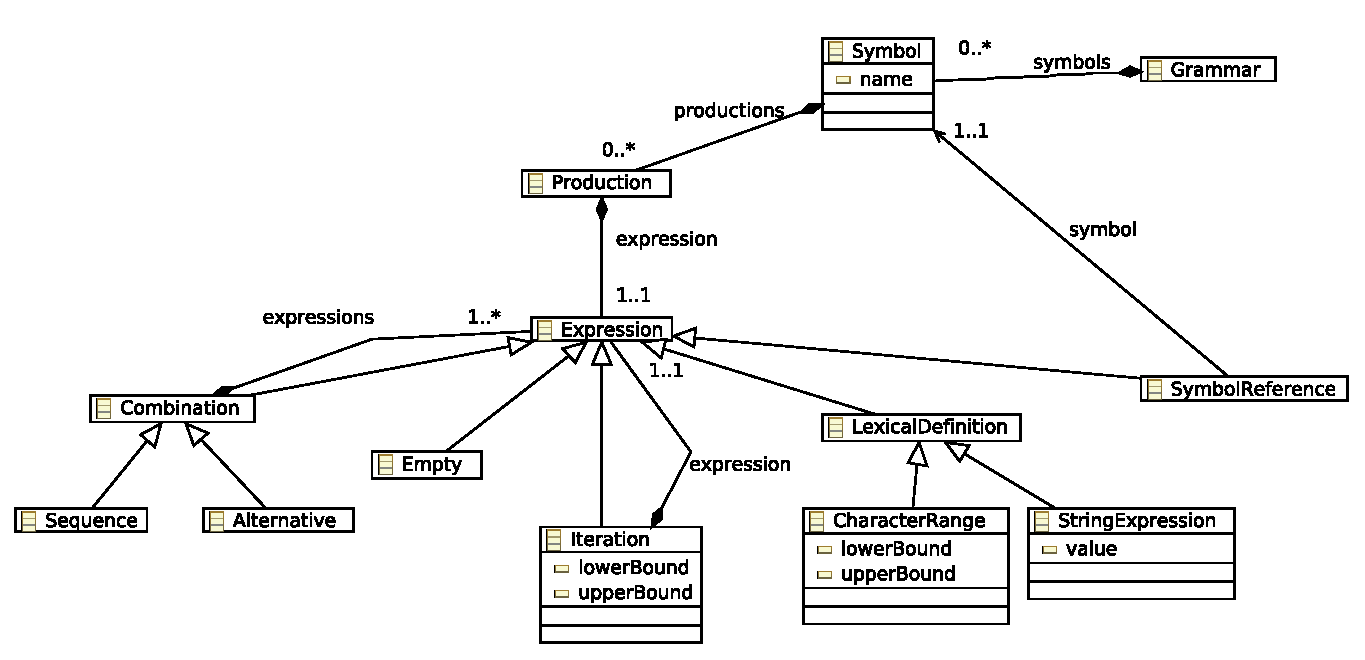
\includegraphics[width=\textwidth]{grammar.pdf}
\caption{Основные элементы мета-модели \tool{Grammatic}}\label{GCore}
\end{figure}

Синтаксис \tool{Grammatic} основан на нотации популярного генератора \tool{ANTLR}, но отличается явным выделением продукций и пустого слова. Проиллюстрируем его использование на примере простого языка, заданного продукциями, представленными на рисунке \figref{ListProd}. Эти продукции описывают списки, состоящие из символов \code{NAME} и \code{INT} (подразумеваются идентификаторы и целые числа), разделенные запятыми. В нотации \GRM{} эти продукции выглядят так:
\begin{lstlisting}
list 
	: list ',' list
	: NAME
	: INT ;
\end{lstlisting}
Как видно из примера, левая и правая части продукции отделяются друг от друга двоеточием, причем символ в левой части пишется один раз для всех продукций. Тот же язык можно описать, используя операцию ``\code{*}'', что позволяет избежать неоднозначности:
 \begin{lstlisting}
list : item (',' item)* ;
item
	: NAME
	: INT ;
\end{lstlisting}

\begin{figure}[bhtp]
\newcommand{\gp}[2]{#1 & \rightarrow & #2 \\}
$$
\begin{array}{rcl}
\gp{list}{list \, , \, list}
\gp{list}{\mathit{NAME}}
\gp{list}{\mathit{INT}}
\end{array}
$$
\caption{КС-продукции для языка списков}\label{ListProd}
\end{figure}

В приведенном примере определяются только ``синтаксические правила'' \code{list} и \code{item}. 
В принципе, символы \code{INT} и \code{NAME} ничем не отличаются с точки зрения нотации, однако при традиционном подходе эти символы были бы терминальными. \GRM{} не разделяет символы на терминалы и нетерминалы, поскольку, как говорилось выше, для некоторых алгоритмов разбора это разделение не имеет смысла. Таким образом, все символы в спецификации являются нетерминальными, а терминалы представлены литералами в одинарных кавычках. Несмотря на отсутствие принципиального разделения с точки зрения языка, мы придерживаемся обозначений, разделяющих ``разные'' с нашей точки зрения типы символов: имена терминалов мы пишем заглавными буквами, а нетерминалов~--- начиная со строчной буквы\footnote{Этот способ именования также позаимствован из языка спецификаций ANTLR, в котором он является обязательным.}.

Определения символов \code{INT} и \code{NAME} выглядят так:
\begin{lstlisting}
	INT : DIGIT+;
	NAME : IDEN_START IDEN_PART*;
	DIGIT : ['0'--'9'];
	IDEN_START : ['a'--'z''A'--'Z''_'];
	IDEN_PART : DIGIT | IDEN_START;
\end{lstlisting}
Этот пример иллюстрирует использование различных элементов нотации \tool{Grammatic}. Полный перечень представлен в \tabref{operations}.
\begin{figure}[htbp]
\center
	\begin{tabular}{|c|l|}
	\hline
	\bf Нотация & \bf Значение \\
	\hline
	\code{\#empty} & Пустое выражение \\
	\code{a} & Ссылка на символ a \\
	\code{a b} & Последовательность \\
	\code{a | b} & Альтернатива \\
	\code{a*} & Итерация от 0 до бесконечности \\
	\code{a+} & Итерация от 1 до бесконечности \\
	\code{a?} & Итерация от 0 до 1 \\
	\code{['a'--'z']} & Множество символов от 'a' до 'z' \\
	\code{'abc'} & Строка символов 'abc' \\
	\code{(a | b) c} & Круглые скобки для группировки выражений \\
	\hline
	\end{tabular}
	\caption{Выражения \tool{Grammatic}}\label{operations}
\end{figure}
Еще одним хорошим примером послужит описание нотации \tool{Grammatic} с помощью нее самой, приведенное в Приложении \bad{???}.

\section{Метаданные}

Метаданными называют описательные элементы программ, которые не обрабатываются компилятором, но и не являются комментариями: к ним могут получить доступ дополнительные инструменты, работающие с кодом. По аналогии с \tool{Java} метаданные поддерживаются и в \tool{Ecore}: каждому элементу мета-модели можно сопоставить произвольное количество \term{аннотаций}. В следствие сходства с этими подходами, мы тоже называем аннотации в \tool{Grammatic} метаданными.

Как отмечалось выше, для решения различных задач грамматики необходимо снабжать аннотациями, которые будут позже использоваться генераторами. Типичным примером аннотаций являются семантические действия, но это далеко не единственный пример. Так, для построения программы-форматировщика, добавляющей в текст пробелы и переводы строк для того, чтобы текст выглядел ``структурно'', правила форматирования также задаются в виде аннотаций к грамматике, но не содержат инструкций для вычисления каких-либо атрибутов (подробно эта задача будет рассмотрена ниже в этой главе). То же касается и многих других типичных задач, связанных с созданием интегрированных сред разработки: подсветкой синтаксиса, сворачиванием блоков, построением визуального представления структуры программы и т.д. Заранее предвидеть все возможные применения системы нельзя, поэтому \tool{Grammatic} предоставляет гибкий механизм для описания аннотаций произвольной сложности.

Аннотации могут быть присоединены к любому элементу грамматики: символу, продукции, выражению или всей грамматике целиком. Каждая аннотация представляет из себя набор пар ``имя-значение''. В текстовом синтаксисе это оформляется с помощью фигурных скобок:
\begin{lstlisting}
	s{a = 10} 
		: {b = 'abc'} 
		  (e{c = asd})* { d = {x = 5; y = 6} };	
\end{lstlisting}
Пары ``\code{имя = значение}'' мы будем называть \term{атрибутами}\footnote{Использование этого термина может вызвать путаницу с атрибутами в АТГ, но в нашем изложении из контекста всегда будет понятно, о каких атрибутах идет речь.}. В приведенном примере 
\begin{itemize}
\item атрибут \code{a} сопоставлен с символом \code{s} и имеет значение \code{10} (целое число); 
\item атрибут \code{b} сопоставлен с продукцией (такие аннотации пишутся сразу после двоеточия, начинающего продукцию) и имеет значение \code{'abc'} (строка);
\item атрибут \code{с} сопоставлен с вхождением символа \code{e} в правую часть продукции (а не с самим символом!) и имеет значение \code{abc} (идентификатор);
\item атрибут \code{d} сопоставлен с выражением \code{e*} и имеет значение \code{{x = 5; y = 6}} (аннотация, состоящая из двух атрибутов).
\end{itemize}
\begin{figure}[htbp]
\center
	\begin{tabular}{|c|l|}
	\hline
	\bf Нотация & \bf Значение \\
	\hline
	\code{'abc'} & Строка \\
	\code{10} & Целое число \\
	\code{abc} & Идентификатор \\
	\code{\{ a = b; c = 10\}} & Аннотация \\
	\code{ \{\{ a, b, c ; \}\} } & Последовательность \\
	\code{ <{<} s | (a b)* {>}> } & Грамматическое выражение \\
	\hline
	\end{tabular}
	\caption{Предопределенные типы значений атрибутов}\label{valtypes}
\end{figure}
Предопределенные типы значений, приведенные в \tabref{valtypes}, позволяют создавать довольно сложные аннотации. Наибольшую свободу предоставляет тип ``Последовательность'', значения которого являются последовательностями значений других типов и знаков препинания. Ниже мы увидим, как с помощью таких атрибутов можно создавать небольшие ``предметно-ориентированные языки'' внутри \tool{Grammatic}. Если предопределенных типов не хватает, \GRM{} позволяет определять пользовательские типы значений.

В качестве первого содержательного примера использования метаданных рассмотрим описание ассоциативности и приоритетов бинарных операций. Такая функциональность актуальна для генераторов восходящих анализаторов: она позволяет разрешать конфликты в грамматике. Рассмотрим описание грамматики простых арифметических выражений с операциями ``+'' и ``*''. Чтобы указать приоритеты операций, используем атрибут \code{left}, указывающий на левую ассоциативность:
\begin{lstlisting}
expr
	: expr '*'{left=2} expr
	: expr '+'{left=1} expr
	: INT ;
\end{lstlisting}
Генераторы трансляторов семейства \tool{Yacc} требуют указания ассоциативности и приоритетов не индивидуально для каждого вхождения операции, а один раз для всей грамматики. Конвертер может сгененировать такое объявление по спецификации, приведенной выше, но есть и другой вариант: указывать приоритеты в аннотации, сопоставленной всей грамматике:
\begin{lstlisting}
{
	binaryOperations = {{
		left '*' 2;
		left '+' 1;
	}}
}
expr
	: expr '*' expr
	: expr '+' expr
	: INT ;
\end{lstlisting}
Из примера видно, как тип значения атрибута ``Последовательность'' используется для создания встроенного предметно-ориентированного языка. Разбор этого языка должен выполнять конвертер.

Аналогично могут быть указаны семантические действия. В простейшем случае это просто строковые атрибуты, сопоставляемые продукциям (символ ``\code{@}'' используется для сопоставления аннотации текущей продукции):
\begin{lstlisting}
expr
	: expr '*' expr @{code='$1 * $2'}
	: expr '+' expr @{code='$1 + $2'}
	: INT @{code='strToInt($1)'};
\end{lstlisting}%$

В некоторых случаях атрибут играет роль флага: его значение не важно, а роль играет только наличие или отсутствие атрибута. В таких случаях значение атрибута можно не указывать: указывается только имя (без знака равенства). Например, при генерации трансляторов удобно помечать некоторые символы грамматики (как правило ``терминальные'') как элементы форматирования (whitespace) --- чтобы анализатор их игнорировал. Это актуально не только для настоящих символов форматирования (пробелов, переводов строк, табуляции), но и для комментариев. Для такой реализации пометки достаточно указать атрибут без значения:
\begin{lstlisting}
	WS{ignore} : [0x0000-0x0020];
\end{lstlisting}
Заметим, что имя атрибута, которое нужно указать, зависит от конкретного генератора, для которого пишется спецификация. Семантика языка \tool{Grammatic} никак не интерпретирует атрибуты.

Поскольку в одной грамматике могут встречаться атрибуты, предназначенные для разных генераторов, необходимо обеспечить уникальность имен, чтобы атрибуты не ``накладывались''. Это достигается с помощью введения \term{пространств имен} для атрибутов. Пространство имен идентифицируется однородным идентификатором ресурса (Uniform Resource Identifier, URI \cite{uri}), внутри данной грамматики для удобства ему присваивается локальное имя, это делается с помощью директивы \code{namespace}:
\begin{lstlisting}
	namespace example 'http://example.com/Namespace/Example';
\end{lstlisting}
Для нужд самого \tool{Grammatic} выделено системное пространство имен \code{system} с URI ``\code{grammatic:/}''. По умолчанию все атрибуты определяются в системном пространстве имен. Чтобы указать другое пространство имен, используется квалифицированное имя атрибута, например:
\begin{lstlisting}
	A{example.size = 10}
\end{lstlisting}
Различные генераторы должны определять свои пространства имен, чтобы избегать наложения атрибутов.

\section{Пример: язык для описания конечных автоматов}

Для демонстрации возможностей \tool{Grammatic} ниже мы будем использовать предметно-ориентированный язык StateMachine, предложенный М. Фаулером \cite{StateMachine} и широко используемый в литературе по ПОЯ (см., например,~\cite{Zdun}). В данном разделе мы приводим неформальное описание этого языка, дающее представление о его назначении и содержании.

Язык StateMachine позволяет описывать простые конечные автоматы, допускающие только действиями в состояниях, но не на переходах. Целевая мета-модель этого языка представлена на \figref{SMMM}.

\begin{figure}[htbp]
	\centering
	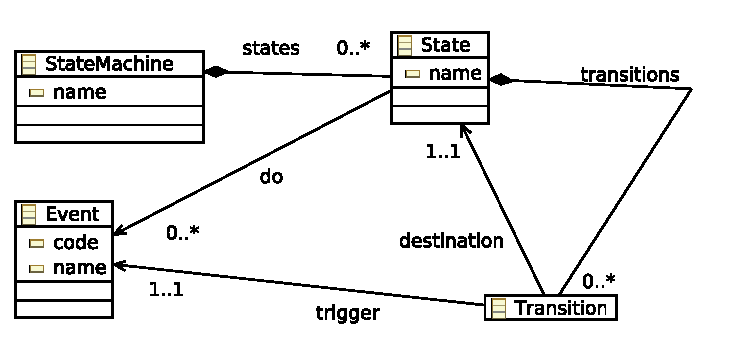
\includegraphics[width=.6\textwidth]{statemachine.pdf}
	\caption{Целевая мета-модель языка StateMachine}\label{SMMM}
\end{figure}

В графической состояния изображаются вершинами графа, переходы --- направленными ребрами (см. \figref{SM}). В вершинах над горизонтальной чертой пишется уникальный идентификатор состояния, а под чертой --- выходные воздействия, генерируемые в этом состоянии. На переходах пишутся входные воздействия, их инициирующие.

\begin{figure}[htbp]
	\centering
	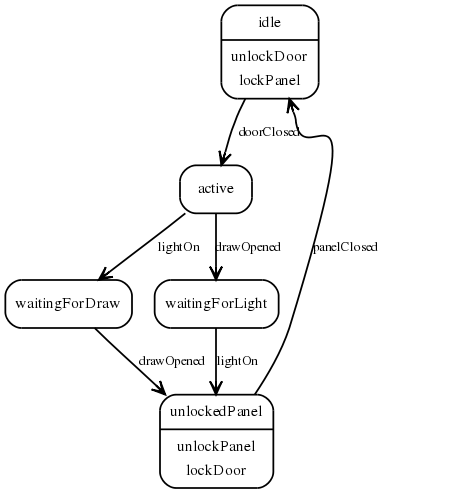
\includegraphics[scale=.5]{smgraph.png}
	\caption{Графическая нотация для языка StateMachine (из \cite{StateMachine})}\label{SM}
\end{figure}

В текстовой нотации автомат описывается с помощью ключевого слова \code{statemachine}, за которым следуем имя автомата и набор состояний в фигурных скобках. Пример использования текстовой нотации приведен в \lstref{SMText}. Cостояния описываются с помощью ключевого слова \code{state}; внутри состояния может находиться блок \code{do}, содержащий последовательность выходных воздействий, а также переходы, описываемые с помощью конструкции \code{on INPUT goto STATE}, где \code{INPUT} --- входное воздействие, а \code{STATE} --- состояние, в которое осуществляется переход.

Входные и выходные воздействия описываются вне блока \code{statemachine} с помощью ключевого слова \code{event}; каждое воздействие имеет уникальное имя и целочисленный код.

\begin{lstlisting}[label=SMText,float=htbp,caption=Текстовая нотация языка StateMachine]
event lockDoor 0; event unlockDoor 1;
event lockPanel 2; event unlockPanel 3;
event doorClosed 4; event doorOpened 5;
event lightOn 6; event drawOpened 7;
event panelClosed 8;

statemachine SecretCompartment {
	state idle {
		do {
			unlockDoor;
			lockPanel;
		}
		on doorClosed goto active;
	}
	state active {
		on lightOn goto waitingForDraw;
		on drawOpened goto waitingForLight;
	}
	state waitingForDraw {
		on drawOpened goto unlockedPanel;
	}
	state waitingForLight {
		on lightOn goto unlockedPanel;
	}
	state unlockedPanel {
		do {
			unlockPanel;
			lockDoor;
		}
		on panelClosed goto idle;
	}
}
\end{lstlisting}

Синтаксические правила языка StateMachine, выраженные в нотации \tool{Grammatic}, приведены в \lstref{SMGram}.

\begin{lstlisting}[xleftmargin=1cm,float=htbp,label=SMGram,caption=Грамматика языка StateMachine]
WS : [0x0000-0x0020];
COMMENT : '//' [^'\n']*;
DIGIT : ['0'-'9'];
NAME_START : ['a'-'z''A'-'Z'_];
NAME_PART : NAME_START | DIGIT;
NAME : NAME_START NAME_PART*;
INT : DIGIT*;

system : event* stateMachine;
stateMachine : 'statemachine' NAME '{' state* '}';
state : 'state' NAME '{' do? (transition ';')* '}';
do : 'do' block;
transition : 'on' eventRef 'goto' stateRef;
stateRef : NAME;
block : '{' (commandRef ';')* '}';
eventRef : NAME;
commandRef : NAME;
event : 'event' NAME INT;
\end{lstlisting}

\chapter{Модули}

Поддержка модулей позволяет разработчику разделять спецификацию на несколько отдельных файлов и при необходимости использовать определения из одного файла повторно.  С точки зрения целевой мета-модели \tool{Grammatic}, модулю соответствует грамматика, определенная в отдельном файле. В данном разделе мы подробно опишем механизм работы таких модулей.

\section{Цитирование и переименование}

Для описания модулей в \tool{Grammatic} не применяется никаких специальных синтаксических конструкций, поэтому файл, содержащий описание грамматики, уже является модулем. Для того, чтобы использовать один модуль внутри другого, применяется директива цитирования \tool{import}, синтаксис которой можно проиллюстрировать на следующем примере:
\begin{lstlisting}
import 'a/b/c/d.grammar' {A, B as C};

B : A C*;
\end{lstlisting}  
Директива \code{import} принимает два аргумента: идентификатор импортируемого файла в одинарных кавычках и список импортируемых символов в фигурных скобках. 

Идентификатором файла является его имя в \term{виртуальной файловой системе}, конфигурация которой подается на вход транслятору \tool{Grammatic} вместе с файлом основной грамматики. В простейшем случае (пустая конфигурация) виртуальная файловая система в точности соответствует физической, и идентификатором файла является просто путь на диске. Однако при использовании библиотек привязка к путям в физической файловой системе приводит к трудностям с переносимостью, поэтому виртуальная файловая система может предоставлять абстрактное представление физической, самостоятельно находя библиотечные модули. Подробнее формат описания виртуальной файловой системы разобран в Приложении \bad{???}.

Список импортированных символов указывается явно для того, чтобы подчеркнуть характер зависимости данного модуля от подключаемого. При необходимости импортировать все символы, список можно заменить знаком \code{\{*\}}.

Ключевое слово \code{as} используется в случае необходимости импортировать символ под другим именем. Так в нашем примере символ \code{B} переименовать необходимо, поскольку в импортирующем модуле определен символ с таким именем. В результате, правило, описанное здесь соответствует диаграмме на \figref{GRenaming}.

\begin{figure}[htbp]
	\centering
	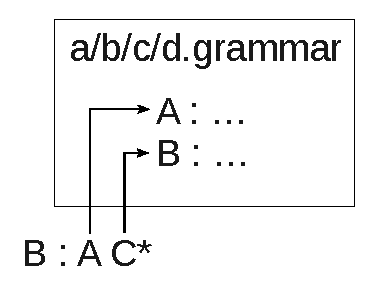
\includegraphics[width=.5\textwidth]{renaming.pdf}
	\caption{Иллюстрация результата переименования}\label{GRenaming}
\end{figure}

Другая форма директивы цитирования позволяет назначить имя самому импортируемому модулю и обращаться к его элементом с помощью квалифицированных имен:
\begin{lstlisting}
import 'a/b/c/d.grammar' as D;

B : D.A D.B*;
\end{lstlisting}  
Заметим, что при трансляции данного примера результат будет идентичным предыдущему, поскольку в правиле для символа \code{B} мы использовали те же символы из подключаемого модуля (\code{A} и \code{B}) в тех же позициях.

\section{Атрибуты доступа}

Нотация \tool{Grammatic} не предусматривает специальных средств для обозначения атрибутов доступа для правил. Тем не менее, соответствующую функциональность обеспечивают специальные атрибуты \code{private} и \code{public}, зарезервированные для этих целей в системном пространстве имен.

\tool{Grammatic} проверяет наличие атрибута \code{private}, и если он есть, запрещает импортировать символ или использовать его квалифицированное имя. Атрибут \code{public} определен для симметрии, и его можно не указывать. Так, в следующем примере недоступен другим модулям только символ \code{C}:
\begin{lstlisting}
A{public} : B C;
B : C;
C{private} : 'c'
\end{lstlisting}  

\section{Модульная грамматика для языка StateMachine}\label{ModularSMG}

В качестве примера, разделим на модули грамматику языка StateMachine, приведенную в \lstref{SMGram}. Первый модуль \code{smlexer.grammar} будет содержать ``лексические'' определения, которые будут использованы в других модулях:
\begin{lstlisting}
// smlexer.grammar
WS{private} : [0x0000-0x0020];
COMMENT{private} : '//' [^'\n']*;
DIGIT{private} : ['0'-'9'];
NAME_START{private} : ['a'-'z''A'-'Z'_];
NAME_PART{private} : NAME_START | DIGIT;
NAME : NAME_START NAME_PART*;
INT : DIGIT*;
\end{lstlisting}
Заметим, что доступными извне являются только символы \code{INT} и \code{NAME}, поскольку все остальные символы носят служебный характер.

Основные синтаксические правила мы разделим на два модуля: \code{smmain.grammar}, определяющий структуру автомата, и \code{smevents.grammar}, описывающий входные и выходные воздействия:
\begin{lstlisting}
// smmain.grammar

import 
	'smlexer.grammar' {NAME},
	'smevents.grammar' {*};

system : event* stateMachine;
stateMachine : 'statemachine' NAME '{' state* '}';
state : 'state' NAME '{' do? (transition ';')* '}';
do : 'do' block;
transition : 'on' eventRef 'goto' stateRef;
stateRef : NAME;
block : '{' (commandRef ';')* '}';

// smevents.grammar
import 
	'smlexer.grammar' {NAME, INT};
	
eventRef : NAME;
commandRef : NAME;
event : 'event' NAME INT;
\end{lstlisting}
Данный пример демонстрирует возможность повторного использования модуля \code{smlexer.grammar}.

\chapter{Шаблоны}

Как отмечалось выше, шаблоны (макроопределения) позволяют повторно использовать фрагменты грамматики, внося в них некоторые изменения, посредством подстановки на место параметров шаблона реальных значений. Например, если в нотации языка StateMachine мы бы хотели сделать последнюю точку с запятой в списках выходных воздействий и переходов необязательной (как в языке Pascal), нам пришлось бы дважды написать относительно запутанное выражение:
\begin{lstlisting}
state : 'state' NAME '{' do? 
			(transition (';' transition)* ';'?)* 
		'}';
block : '{' 
			(commandRef (';' commandRef)* ';'?)* 
		'}';
\end{lstlisting}

В грамматиках больш\'{и}х языков повторения подобных конструкций могут встречаться десятки раз. Чтобы избежать дублирования, можно определить шаблон вида ``\code{элемент~(разделитель~элемент)*~разделитель?}'', и применить его дважды, подставляя разные значения вместо параметров ``\code{разделитель}'' и ``\code{элемент}'', что позволяет сократить длину кода, улучшить его читаемость и уменьшить вероятность появления ошибок.

В нотации \tool{Grammatic} шаблоны объявляются следующим образом:
\begin{lstlisting}[xleftmargin=.5cm]
template List<item : Expression, sep : Expression> : Expression {
	<?item> (<?sep> <?item>)* <?sep>?
}
\end{lstlisting}
Первая строка определяет \term{сигнатуру шаблона}, как мы покажем ниже, она используется для гарантий структурной корректности результатов применения шаблона. После двоеточия указывается тип параметра (или результата). Типы соответствуют классам мета-модели \code{Grammatic} (см. \figref{GCore}). Часто (в частности, в данном примере) типы можно опускать, поскольку транслятор способен определить их самостоятельно. В целом, шаблон напоминает функцию: у него есть имя, аргументы и возвращаемое значение; единственное отличие состоит в том, что при применении шаблона результат вычисляется транслятором статически, а не ``во время выполнения''\footnote{Что такое ``время выполнения'' для языка \code{Grammatic} не вполне ясно, тем не менее, что понятие ``статическиого вычисления'' не вызывает сомнений: такие вычисления выполняются транслятором в процессе вычисления функции $Meaning$.}. Аналогично функциям, чтобы использовать ранее определенный шаблон, нужно указать его имя и параметры:
\begin{lstlisting}
state : 'state' NAME '{' do? 
			<List transition, ';'>
		'}';
block : '{' 
			<List commandRef, ';'>
		'}';
\end{lstlisting}
Содержание этого определения символов \code{state} и \code{block} идентично приведенному выше.

Теперь приступим к более детальному описанию механизма шаблонов в \tool{Grammatic}.

\section{Элементы языка шаблонов}
Целевая мета-модель, описывающая шаблоны, приведена на \figref{TempMM}.

\begin{figure}[htbp]
	\centering
	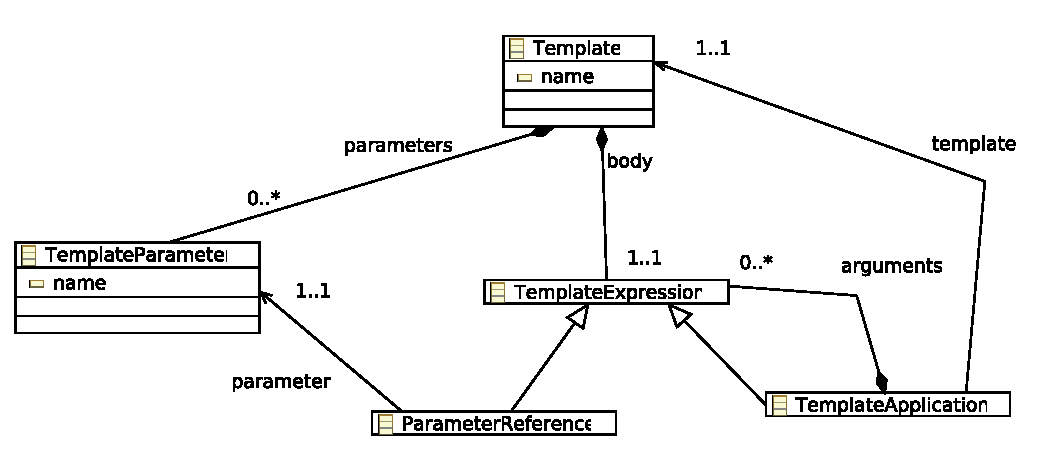
\includegraphics[width=.6\textwidth]{template.pdf}
	\caption{Целевая мета-модель языка шаблонов}\label{TempMM}
\end{figure}

Добавляя шаблоны в язык, мы расширяем основную нотацию, добавляя новые конструкции так, чтобы получившуюся нотацию можно было транслировать в исходную. Можно считать, что мы создаем новый язык: на основе уже описанного языка грамматик строим языка шаблонов грамматик.

В этом новом языке центральным понятием является \term{шаблонное выражение}: то, что может являться телом шаблона. На \figref{TempMM} шаблонным выражениям соответствуют классы-наследники \code{TemplateExpression}. Простейшие шаблонные выражения --- это константы, то есть обычные выражения языка описания грамматик, не содержащие шаблонных параметров и обращений к шаблонам. Например, выражение \code{A B* | C}, как и все его подвыражения, является примером такой константы. Таким образом, нотация для шаблонных выражений включает в себя нотацию для грамматик как подмножество. Заметим, что шаблонные выражения имеют типы, соответствующие классам в целевой мета-модели языка грамматик.

Новыми элементами в нотации шаблонных выражений являются обращения к шаблонным параметрам (класс \code{ParameterUsage}), которые записываются в угловых скобках (\code{A <?paramName>* | C}), и вызовы шаблонов (класс \code{TemplateApplication}), которые также заключаются в угловые скобки, но, кроме имени, содержат также список аргументов шаблона, разделенных запятыми:
\begin{lstlisting}
	<List expression, ';'>
\end{lstlisting}

Шаблонные выражения записываются внутри объявлений шаблонов (класс \code{Template}), и представляют собой \term{тело} шаблона. Синтаксически объявление шаблона оформляется с помощью ключевого слова \code{template}:
\begin{lstlisting}[xleftmargin=.5cm]
template List<item : Expression, sep : Expression> : Expression {
	<?item> (<?sep> <?item>)* <?sep>?
}
\end{lstlisting}
Как мы отмечали выше, типы, указанные в объявлении, используются для гарантий корректности результата применения данного шаблона. Шаблонные параметры, описанные в сигнатуре шаблона, могут быть использованы только в его теле. Объявления шаблонов не вкладываются одно в другое, также не допускаются рекурсивные вызовы шаблонов (прямые или косвенные), поскольку вычисление значения при вызове такого шаблона никогда не закончится.

Типы, используемые при объявлении шаблонов строятся по следующим правилам: 
\begin{itemize}
\item \term{Элементарные типы} --- это классы мета-модели грамматик (\code{Expression}, \code{Sequence}, \code{Production}, \code{Symbol} и т.д.).
\item \term{Составные типы} образуются из элементарных следующими операциями:
	\begin{itemize}
		\item ``?'' значение элементарного типа является необязательным;
		\item ``+'' непустой список значений элементарного типа;
		\item ``*'' произвольный список значений элементарного типа.
	\end{itemize}
\end{itemize}

\section{Примеры использования шаблонов}

Выше мы показали, как и для чего могут быть использованы шаблоны отдельных выражений. Для таких целей шаблоны применяются в EBNF \cite{EBNF} и \tool{Menhir} \cite{Menhir}. В Главе \ref{part1} мы также описывали параметризованные модули, используемые в \tool{ASF+SDF} и \tool{Rats!}, в данном разделе мы покажем, как шаблоны \tool{Grammatic} позволяют реализовать аналогичную функциональность. Кроме того, мы покажем, что можно использовать и шаблоны метаданных.

\subsection{Параметризованные модули}

Мы разработаем вариант описания языка StateMachine, который позволит нам варьировать содержание понятий входного и выходного воздействия. В разделе \ref{ModularSMG} мы выделили три модуля в грамматике языка StateMachine, один из которых, \code{smevents.gramar} содержал определения для символов \code{even}, \code{eventRef} и \code{commandRef}, которые использовались в главном модуле. Такая реализация уже позволяет изменять определения данных символов, не изменяя кода главного модуля, но она не позволяет использовать \term{параллельно} два варианта реализации понятия ``воздействие''. Для того, чтобы поддержать эту возможность, мы видоизменим главный модуль, введя шаблонные параметры:
\begin{lstlisting}
// smmain.grammar

import 
	'smlexer.grammar' {NAME};

template SMMain<event : Expression, eventRef : Expression, 
		commandRef : Expression> : Symbol+ 
{
	system : <?event>* stateMachine;
	stateMachine : 'statemachine' NAME '{' state* '}';
	state : 'state' NAME '{' do? (transition ';')* '}';
	do : 'do' block;
	transition : 'on' <?eventRef> 'goto' stateRef;
	stateRef : NAME;
	block : '{' (<?commandRef> ';')* '}';
}
\end{lstlisting}
Важно заметить, что модуль \code{smevents.grammar} больше не используется, а вместо обращений к символам этого модуля введены шаблонные параметры.

Теперь определим два сосуществующих варианта описания входных и выходных воздействий: первый --- тот, что уже использовался, а второй --- позволяющий сопоставить каждому воздействию строку для записи в журнал событий. Первый вариант реализует уже знакомый нам модуль \code{smevents.grammar}:
\begin{lstlisting}
// smevents.grammar
import 
	'smlexer.grammar' {NAME, INT};
	
eventRef : NAME;
commandRef : NAME;
event : 'event' NAME INT;
\end{lstlisting}
Второй вариант мы реализуем в модуле \code{smevents-log.grammar}:
\begin{lstlisting}
// smevents-log.grammar
import 
	'smlexer.grammar' {NAME, INT};
	
logEventRef : NAME;
logCommandRef : NAME;
logEvent : 'event' NAME INT STRING?;

STRING : '\'' [^'\'''\n''\r']* '\'';
\end{lstlisting}

Теперь необходимо соединить каждую из этих реализаций с главным модулем. Для этого достаточно применить определенный этим модулем шаблон и передать соответствующие параметры. Для первого случая получим
\begin{lstlisting}
<SMMain event, eventRef, commandRef>
\end{lstlisting}
Для второго случая получим
\begin{lstlisting}
<SMMain logEvent, logEventRef, logCommandRef>
\end{lstlisting}
Шаблоны делают данные определения гораздо компактнее: если бы нам пришлось обходиться обычными модулями, определение главного модуля пришлось бы записать дважды --- по одному разу для каждого варианта реализации воздействий.

\subsection{Шаблоны метаданных}

Поскольку метаданные тоже входят в основную нотацию \tool{Grammatic}, можно создавать и шаблоны аннотаций. В основном, такие шаблоны понадобятся нам для реализации механизма аспектов, а в этом разделе мы приведем простой пример, показывающий, как с их помощью можно регламентировать структуру аннотаций.

Генератор документации для грамматик использует метаданные как источник дополнительной информации: специальные атрибуты хранят текст, описывающий назначение символа, примеры строк, которые он выводит и т.д. Для примера приведем описание оператора \code{if} некоторого гипотетического языка:
\begin{lstlisting}[xleftmargin=0.3cm]
if
{	doc.title = 'Conditional operator';
	doc.description = 
'If expression evaluates to true, <pre>then</pre> branch is taken,
otherwise -- <pre>else</pre> branch is taken';
	doc.examples = {{
		'if a > 1 then WriteLn(a)'
		'if (x < 0) and (x > -5) then x := -x else x := 2 * x'
	}}
} : 'if' expression 'then' statement ('else' statement) ;
\end{lstlisting}

Из такого описания генератор построит следующий текст:
\begin{center}
\fbox{
\parbox{0.7\textwidth}{
{{\bf Conditional operator}\\
\small
{\bf Syntax}: \\
\textit{if} ::= \texttt{if} \textit{expression} \texttt{then} \textit{statement} \texttt{else} \textit{statement}\\
{\bf Description}: 
If expression evaluates to true, \texttt{then} branch is taken,
otherwise -- \texttt{else} branch is taken\\
{\bf Examples}: 
\begin{itemize}
\item \textbf{if} a > 1 \textbf{then} WriteLn(a)
\item \textbf{if} (x < 0) \textbf{and} (x > -5) \textbf{then} x := -x \textbf{else} x := 2 * x
\end{itemize}
}}}
\end{center}

Мы используем шаблон аннотации для того, чтобы гарантировать, что разработчик укажет все атрибуты, необходимые для генерации документации:
\begin{lstlisting}
template Doc<title : String, description : String, 
	examples : String+> : Attribute+ 
{
	doc.title = <?title>;
	doc.description = <?description>;
	doc.examples = {{ <?examples> }};
}
\end{lstlisting}
С применением этого шаблона метаданные для символа \code{if} будут выглядеть так:
\begin{lstlisting}[xleftmargin=0.6cm]
if
{Doc<
'Conditional operator',
'If expression evaluates to true, <pre>then</pre> branch is taken,
otherwise -- <pre>else</pre> branch is taken',
'if a > 1 then WriteLn(a)',
'if (x < 0) and (x > -5) then x := -x else x := 2 * x'
>} : 'if' expression 'then' statement ('else' statement) ;
\end{lstlisting}
В этом случае \tool{Grammatic} выдаст сообщение об ошибке, если один из элементов документации не будет указан.

\chapter{Аспекты}%
%
Еще одним механизмом композиции, реализованным в \tool{Grammatic} являются аспекты. Как мы отмечали выше, этот механизм обеспечивает выполнение двух основополагающих свойств:
\begin{itemize}
\item \term{Незнание} --- отсутствие необходимости специальным образом обозначать или иначе подготавливать участок программы, в который будет внесено изменение с помощью аспектов. Другими словами, наличие аспекта не влияет на структуру программы, в которую он встраивается, то есть программа \term{не знает} о существовании аспекта.
\item \term{Квантификация} --- возможность встроить один и тот же совет в несколько участков программы, описанных некоторым выражением. Это выражение играет роль \term{квантора} (аналогично квантору всеобщности в логике предикатов \cite{???}).
\end{itemize}

Незнание достигается за счет композиционных свойств семантики аспектов: встраивание преобразует одну корректную программу в другую корректную программу, не требуя от исходной программы никаких специальных свойств. Все обязательства по обеспечению совместимости берет на себя аспект.

Квантификация достигается с помощью механизма \term{срезов} (point-cuts) --- специальных выражений, которые описывают множества \term{точек встраивания} (join points). Далее \term{советы} (advice) ассоциируются не с отдельными точками встраивания, а со срезами, что позволяет избежать дублирования советов.

\section{Основные понятия АОП в \tool{Grammatic}}

В следующих подразделах мы покажем как эти общие положения АОП реализуются в \tool{Grammatic}, и как они могут быть использованы для достижения модульности грамматик, отделения семантики языков от синтаксиса и сокращения дублирования кода при автоматической генерации сред разработки.

\subsection{Точки встраивания и срезы}

Точками встраивания в \tool{Grammatic} являются все элементы грамматики: символы, продукции, выражения, аннотации и т.д. Таким образом, с помощью аспектов можно модифицировать любые структуры внутри грамматики. Такое решение требует от языка срезов достаточно большой выразительной силы: срезы должны позволять выбирать из грамматики объекты довольно сложной структуры.

Срезы напоминают язык регулярных выражений над грамматиками; они представляют собой образцы для сопоставления с конструкциями в грамматике. Самой простой формой среза является константный срез, то есть образец, который в точности повторяет фрагмент грамматики, с которым он сопоставляется. Фактически, этот вид среза представляет собой прямую цитату из грамматики, например:
\begin{lstlisting}
a : b | c d* ;
\end{lstlisting}
Этот образец успешно сопоставляется только с правилом грамматики, которое записывается в точности так же. Таким образом, срезы, как и шаблоны, включают те же базовые элементы, что и грамматики (см. \figref{operations}). Срезы дополняют этот набор элементов \term{подстановочными знаками} (wildcards).

Подстановочные знаки аналогичны символу ``.'' в стандартных регулярных выражениях, но, поскольку элементы грамматик являются типизированными, подстановочные знаки позволяют различать типы. Обобщенный подстановочный знак можно записать как ``\code{<? : тип>}''. Так, например, выражение, описывающее последовательность любых элементов, заключенных в скобки, будет успешно сопоставлено со следующим образцом:
\begin{lstlisting}
'(' <? : Sequence> ')'
\end{lstlisting}
Например, если мы сопоставим с этим образцом выражение \code{'(' a* b ')'}, сопоставление пройдет успешно, поскольку с посдстановочным знаком будет сопоставлена последовательность \code{a* b}.

Для того, чтобы обращаться к фрагментам сопоставляемых выражений, в срезах можно использовать \term{переменные}. Рассмотрим пример:
\begin{lstlisting}
?seqInBrack=('(' ?s=<? : Sequence> ')')
\end{lstlisting}
Этот образец будет успешно сопоставлен с выражением \code{'(' a* b ')'}, и с переменными будут связаны следующие значения:
\begin{itemize}
\item \code{s = a* b};
\item \code{seqInBrack = '(' a* b ')'}.
\end{itemize}

Каждое имя может быть определено ровно один раз внутри одного образца. Ранее определенную переменную можно \term{использовать} в том же образце, например:
\begin{lstlisting}
?s=<? : Sequence> (<? : Sequence> ?s)*
\end{lstlisting}
Приведенный пример успешно сопоставляется с выражениями \code{a (',' a)*} и \code{'?' var ('-' '?' var)*}, при этом в первом случае c переменной \code{s} связывается значение \code{a} (один элемент тоже является последовательностью), а во втором --- \code{'?' var}. Использовать переменную внутри ее собственного определения нельзя.

Все объекты, связанные с данной переменной будут структурно идентичны. Для переменных, определенных с помощью знака ``='' также можно указывать типы, например:
\begin{lstlisting}
?(seqInBrack : Sequence)=('(' ?(s : Sequence)=<? : Sequence> ')')
\end{lstlisting}
Тип выражения в правой части должен быть подтипом для типа переменной. 

Для упрощения работы с подстановочными знаками, для некоторых типов введены короткие обозначения, приведенные в \tabref{ShortWildcards}.
\begin{figure}[htbp]
	\centering
	\begin{tabular}{|c|l|}
	\hline  \bf Короткая запись & \bf Значение \\ 
	\hline  
	\code{..}  & \code{<? : Sequence>} \\ 
	\code{...}  & \code{<? : Alternative>} \\ 
	\code{:.:}  & \code{<? : Production>} \\ 
	\code{\#}  & \code{<? : Symbol>} \\ 
	\code{\#lex}  & \code{<? : LexicalDefinition>} \\ 
	\code{\{*\}}  & \code{<? : Attribute*>} \\ 
	\hline 
	\end{tabular} 
	\caption{Короткие обозначения для подстановочных знаков}\label{ShortWildcards}
\end{figure}
С их помощью выражение ``\code{?s=<? : Sequence> (<? : Sequence> ?s)*}'' можно записать в следующей форме:
\begin{lstlisting}
?s=.. (.. ?s)*
\end{lstlisting}

\subsection{Советы}

Срезы обеспечивают ``адресацию'' в грамматике и позволяют выбрать позиции для встраивания советов, то есть для добавления новых элементов или замены существующих. В общем виде это оформляется следующим образом:
\begin{lstlisting}[escapeinside={!}{!}]
!образец! ;
	instead !переменная! : !шаблонное выражение!;
	before  !переменная! : !шаблонное выражение!;
	after   !переменная! : !шаблонное выражение!;
	remove  !переменная!;
\end{lstlisting}
Переменные должны быть связаны в образце. Шаблонные выражения могут использовать все переменные, связанные в образце, как шаблонные параметры. Советы \code{instead} заменяют все вхождения переменной на результат разворачивания шаблонного выражения; советы \code{before} и \code{after} --- вставляют результат разворачивания шаблонного выражения до или после каждого вхождения переменной, соответственно; \code{remove} --- удаляют все вхождения данной переменной. Рассмотрим пример:
\begin{lstlisting}
?i=.. (?sep=#lex ?i);
	instead sep : <?sep>+;
\end{lstlisting}
Образец, использованный в данном примере, успешно сопоставляется с любым списком, где разделителем является содержимое переменной \code{?sep}. Совет \code{instead} помещает разделитель под оператор \code{+}. Например, если данный аспект применить к следующей грамматике:
\begin{lstlisting}
expr : factor ('*' factor)*;
factor : '(' NUM (',' NUM)* ')';
\end{lstlisting}
оба разделителя (\code{*} и \code{,}) будут заменены соответствующим образом, и в результате получится следующая грамматика:
\begin{lstlisting}
expr : factor ('*'+ factor)*;
factor : '(' NUM (','+ NUM)* ')';
\end{lstlisting}

Чтобы, например, добавить перед вхождениями символа \code{NUM} необязательный знак ``--'', достаточно применить следующее аспектное правило:
\begin{lstlisting}
.. ?n=NUM ..;
	before n : '-'?;
\end{lstlisting}
То же преобразование можно выразить с помощью \code{instead}. В действительности, любой совет выражается через \code{instead}.

Аспекты позволяют модифицировать и метаданные. Например, чтобы добавить атрибут к аннотации на данном выражении, можно применить следующий аспект:
\begin{lstlisting}
example : .. ?e=('(' .. ')') .. ;
	instead e : <?e> {a = 10} ;
\end{lstlisting}
Поскольку несколько аннотаций на одном и том же объекте объединяются в одну, данный пример добавляет атрибут, не удаляя уже имеющихся. Чтобы удалить имеющиеся атрибуты, необходимо связать их с некоторой переменной и заменить ее значение пустой аннотацией:
\begin{lstlisting}
example : .. ?e=('(' .. ')')?a={*} .. ;
	instead a : {};
\end{lstlisting}

Как мы покажем ниже советы, добавляющие аннотации к элементам грамматики, имеют большое значение, поэтому поддерживается следующая краткая форма записи:
\begin{lstlisting}
example : .. ?e=('(' .. ')') .. ;
	@e : {a = 10} ;
\end{lstlisting}
Данное правило добавляет атрибут \code{a} ко всем вхождениям переменной \code{e}.

\section{Семантика применения аспектов}

Подробно семантика аспектов и шаблонов описана в Главе \ref{part4} для случая произвольного предметно-ориентированного языка. В этом разделе мы приводим только основные сведения, необходимые для понимания механизма работы аспектов.

Выше были приведены примеры \term{аспектных правил}, объединяющих один срез и несколько советов, определенных для переменных, связанных в этом срезе. Аспект представляет собой набор подобных правил, описанных в одном файле.
Когда аспект применяется в грамматике (это отдельная операция, которую выполняет специальный модуль в библиотеке \GRM{}), для каждого аспектного правила образец сопоставляется со всеми элементами грамматики, и для каждого удачного сопоставления применяются советы.

\GRM{} позволяет контролировать, сколько раз был сопоставлен каждый образец. Для этого перед правилом пишется специальная директива, например:
\begin{lstlisting}
#(0,1) 
example : .. ?e=('(' .. ')') .. ;
	@e : {a = 10} ;
\end{lstlisting}
В скобках указываются минимальное и максимальное допустимое число успешных сопоставлений, так \code{\#(0,1)} означает, что данному образцу должно соответствовать не более одного элемента внутри грамматики, а \code{\#(1,1)}~--- что ровно один. Для обозначения неограниченного числа сопоставлений соответствующее число просто не указывается: \code{\#(1,)}.

\chapter{Применение \tool{Grammatic}}

Как отмечалось выше, \GRM{} интегрируется с существующими инструментами, позволяя использовать мощные механизмы композиции при работе с грамматиками.
В данном разделе мы приводим примеры применения этого языка для описания диалектов языка \tool{SQL} и компонент интегрированной среды разработки. Во втором случае использование аспектов для отделения метаданных от грамматических продукций позволяет повторно использовать грамматики и улучшить их читаемость.

\section{Описание диалектов языка SQL}

Стандарт \tool{SQL-92} \cite{SQL92} охватывает широкий круг возможностей языка, и большинство реализаций поддерживают его лишь частично. Кроме того, некоторые реализации добавляют собственные синтаксические конструкции в язык. При создании инструментов разработки, не привязанных к конкретной реализации СУБД\footnote{Система управления базами данных.} возникает задача компактного описания нескольких диалектов \tool{SQL} для того, чтобы корректно обрабатывать код, написанный для различных реализаций.

В данном разделе описано применение \GRM{} для описания синтаксиса диалектов \tool{SQL} с помощью аспектов, применяемых к грамматике языка, описанной в стандарте. Данная грамматика содержит 961 правило, из них 514 синтаксических (остальные --- лексические), поэтому ни ее, ни даже описания диалектов полностью мы не приводим, но приводим примеры, дающие представление о способе описания и его эффективности.

С помощью \GRM{} спецификация \tool{SQL} была разбита на 17 модулей. В тексте спецификации были обнаружены следующие повторяющиеся конструкции, которые были заменены шаблонами выражений:
\begin{itemize}
\item перестановочные выражения:
\begin{lstlisting}
	template Commute<a, b> {<?a> <?b>? | <?b> <?a>?}
\end{lstlisting}
\item необязательное вхождение выражения в круглых скобках:
\begin{lstlisting}
	template OptParen<a> {('(' <?a> ')')?}
\end{lstlisting}
\item бинарные операции:
\begin{lstlisting}
	template OptParen<symbol, factor, op1, op2> {
		<?symbol>
			: <?factor>
			: <?symbol> op1 <?symbol>
			: <?symbol> op2 <?symbol> ;
	}
\end{lstlisting}
\item список с разделителем:
\begin{lstlisting}
	template OptParen<item, sep> {
		<?item> (<?sep> <?item>)*
	}
\end{lstlisting}
\end{itemize}

Для описания диалектов применяются аспекты. Так документация по СУБД \tool{PostgreSQL} \cite{PostgreSQL} отмечает некоторые отличия в синтаксисе запроса \code{SELECT} по сравнению со стандартом. Опишем эти отличия в виде аспектных правил, применяемых к грамматике \tool{SQL92}: образцы соответствуют стандартному синтаксису, а советы отражают изменения, имеющиеся в диалекте.
%\url{http://www.postgresql.org/files/documentation/books/aw_pgsql/node278.html#SECTION0032784100000000000000}
%optional FROM
%mandatory AS
%The DISTINCT ON phrase is not part of SQL92. Nor are LIMIT and OFFSET. 
%Postgres also allows both clauses (ORDER BY GROUP BY) to specify arbitrary %expressions
%The CORRESPONDING BY clause is not supported by Postgres. 
\begin{itemize}
\item В \tool{PostgreSQL} предложение \code{FROM} является необязательным:
\begin{lstlisting}
tableExpression : ?f=fromClause ..;
	instead f : fromClause?;
\end{lstlisting}
%
\item Использование ключевого слова \code{AS} при указании псевдонима обязательно:
\begin{lstlisting}
asClause : ?a=(AS?) ..;
	instead a : AS;
\end{lstlisting}
%
\item Квантор \code{DISTINCT} может быть снабжен предложением \code{ON}, которое позволяет указать, на каких выражениях необходимо сравнивать результаты запроса, чтобы исключить повторения:
\begin{lstlisting}
setQuantifier : ?d=DISTINCT | ...;
	after d : (ON '(' <List expression ','> ')')?;
\end{lstlisting}
%
\item В предложении \code{GROUP BY} разрешается указывать произвольные выражения:
\begin{lstlisting}
groupingColumnReference : ?p=:.:;
	after p : : valueExpression;
\end{lstlisting}
%
\item Спецификации \code{CORRESPONDING BY} не поддерживаются:
\begin{lstlisting}
nonjoinQueryTerm : ... | (.. ?c=(correspondingSpec?) ..);
	remove P;
\end{lstlisting}
%
\end{itemize}
Как видно из примеров, каждое отличие реализуется весьма кратко, что делает всю спецификацию диалекта компактной. Такая спецификация может быть разделена на аспект, вносящий дополнения в стандартную грамматику, и аспект, удаляющий неподдерживаемые конструкции. Наиболее вероятно, что из второго аспекта правила будут удаляться по мере того, как соответствующие конструкции будут поддерживаться в новых версиях СУБД.

Аналогичные аспектные описания можно сделать и для других диалектов, например, \tool{Derby} \cite{Derby}.
%\url{http://db.apache.org/derby/docs/10.0/manuals/reference/sqlj151.html}
%natural join
%INTERSECT
%Full outer join
%Union join
В целом, механизм аспектов показал себя очень эффективным инструментом для описания семейств родственных языков.

\section{Применение аспектов для отделения метаданных}

В последние годы интегрированные среды разработки для языков общего назначения достигли весьма высокого уровня развития, и минимальные требования пользователей к инструментальной поддержке языков (в том числе и предметно-ориентированных) стали заметно выше. В связи в этим все большую актуальность приобретает задача автоматизации разработки компонент интегрированных средств разработки, таких как модули для
\begin{itemize}
	\item автоматического форматирования кода,
	\item подсветки синтаксиса,
	\item структурного отображения кода и сворачивания блоков,
	\item автодополнения в среде разработки.
\end{itemize}

Некоторые инструменты, например \cite{xText}, позволяют генерировать все эти компоненты по описанию языка, однако генерируемые ими модули трудно настраивать, поскольку разработчики предпочли краткость описания языка мощности генератора. Существуют и более гибкие инструменты, позволяющие генерировать подобные компоненты. Сложность состоит в том, что каждый из этих инструментов генерирует лишь один вид компонент, и ни один не генерирует все. Так с помощью \tool{Pretzel} \cite{Pretzel} можно получать качественные модули для автоматического форматирования, но для этого требуется предоставить грамматику со специальными аннотациями, регламентирующими форматирование. В свою очередь, для подсветки синтаксиса подходят легковесные методы разбора (см. например,~\cite{RegReg}), для использования которых требуется либо переписать грамматику полностью, либо снабдить ее аннотациями, с помощью которых конвертер может сгенерировать соответствующее описание.

Таким образом, возникает следующая ситуация: для того, чтобы получить поддержку нескольких функций среды разработки, нужно предоставить одну и ту же грамматику, но с разными аннотациями. Без использования аспектов эта задача решается одним из двух способов:
\begin{itemize}
\item предоставить несколько копий грамматики с разными аннотациями;
\item предоставить одну грамматику, в которой указаны все необходимые аннотации.
\end{itemize}
Без использования обобщенной нотации, такой как \GRM{}, второй способ реализовать невозможно, а кроме того, смешивание аннотаций различного назначения существенно затрудняет чтение грамматики и внесение изменений.

Первый же способ предполагает дублирование грамматики, что также осложняет поддержку, поскольку при внесении изменений их необходимо вносить во все копии грамматики, а при этом легко допустить ошибку.

Аспекты в \GRM{} предоставляют третий способ: грамматика описывается отдельно, вообще без метаданных, а аннотации присоединяются с помощью аспектов. При этом аннотации можно группировать по назначению: каждый файл с аспектными правилами определяет отдельный \term{аспект} системы. Этот подход соответствует идеологии разделения \term{пересекающихся интересов} (croscutting concerns), на которой основывается аспектно-ориентированное программирование \cite{AOP}.

Приведем примеры аспектных правил для описания автоматического форматирования для языка \tool{Java}, применяемых к грамматике приведенной в стандарте языка \code{JLS}. Для этого используются атрибуты \code{before} и \code{after}, значения которых определяют, какие разделительные символы должны быть вставлены до и после соответствующей языковой конструкции. Значениями этих атрибутов являются последовательности, состоящие из строковых литералов и идентификаторов \code{increaseIndent}~--- для увеличения текущего отступа и \code{decreaseIndent}~--- для уменьшения. Следующее правило регламентирует форматирование содержимого класса: 
\begin{lstlisting}
classBody : ?b=’{’ ?c=classBodyDeclaration* ?e=’}’
    @b: { after = {{ ’\n’ increaseIndent }} } ;
    @c: { after = {{ ’\n’ }} } ;
    @e: {
        before = {{ decreaseIndent }};
        after = {{ ’\n’ }};
    };
\end{lstlisting}
После фигурной скобки следует перевод строки и увеличение отступа, далее после декларации каждого элемента переводится строка, а перед закрывающей фигурной скобкой отступ уменьшается, чтобы она оказалась на одном уровне с заголовком класса.

Для большинства элементов правило форматирования одно и то же: после элемента печатается пробел. Это описывается один раз в аннотации к грамматике:
\begin{lstlisting}
?g=<? : Grammar>;
	@g : {
	    defaultAfter  = {{ ’ ’ }};
    	defaultBefore = {{ ’’ }};
	}
\end{lstlisting}

Для некоторых элементов форматирование по умолчанию приходится отменять:
\begin{lstlisting}
typeParameters : ?b=’<’ ?t=typeParameter (’,’ ?t)* ’>’
    @b: { after = {{ ’’ }} } ;
    @t: { after = {{ ’’ }} } ;
\end{lstlisting}

Аналогично (но с использованием других атрибутов) описываются подсветка синтаксиса и другие функции среды разработки. Хотя отделение аспектов позволяет хранить грамматику в ``чистом'' виде, без аннотаций, образцы в аспектных правилах дублируют части грамматики. Возникает вопрос: есть ли у такого подхода преимущества по сравнению с копированием грамматики. На наш взгляд ответ утвердительный, по следующим причинам:
\begin{itemize}
\item дублируется не вся грамматика, а только некоторые ее части, поскольку не ко всем правилам нужно добавлять аннотации;
\item использование подстановочных знаков позволяет не менять аспекты при изменениях грамматики, что снимает значительную часть затруднений;
\item контроль количества сопоставлений позволяет автоматически отслеживать, было ли применено аспектное правило, вследствие чего, если при внесении изменений в грамматику, аспект не был изменен соответствующим образом, образец не будет успешно сопоставлен, и произойдет ошибка применения аспекта.
\end{itemize}
Таким образом, \GRM{} позволяет существенно улучшить ситуацию при необходимости сгенрировать несколько артефактов по одной грамматике.

\chapter{Сравнение с существующими инструментами}

Результаты сравнения \GRM{} с другими инструментами представлены в \tabref{GrmTable}. Строки таблицы соответствуют тем или иным возможностям, связанным с механизмами композиции. Для сравнения были выбраны девять инструментов, поддерживающих различные механизмы композиции, а также \tool{Yacc/Bison}, очень широко используемое представляющие семейство инструментов.

\begin{table}[htb]
	\centering
\newcommand{\dissonly}[1]{#1}
\newcommand{\hd}[1]{{\begin{sideways}\parbox{25mm}{\tool{#1}}\end{sideways}}}
%{\begin{sideways}\parbox{15mm}{\bf text}\end{sideways}}
{\size{}\noindent
\begin{tabular}{|ll|c|c|c|c|c|c|c|c|c|c|c|c|}
\hline 
&
	&\hd{Yacc/Bison}
	&\hd{ANTLR}
	&\hd{Menhir}
	&\hd{xText}
	&\hd{ASF+SDF}
	&\hd{JastAdd}
	&\hd{AspectG}
	&\hd{Silver}
	&\hd{LISA}
	&\hd{Rats!}
	&\hd{\textbf{Grammatic}}\\
\hline
\dissonly{
\multicolumn{2}{|r|}{\it Ссылка}
	&\cite{BisonBook}
	&\cite{ANTLR}
	&\cite{Menhir}
	&\cite{xText}
	&\cite{ASF+SDF}
	&\cite{JastAdd}
	&\cite{AspectG}
	&\cite{Silver}
	&\cite{LISA}
	&\cite{Rats!}
	&\\
\hline 
}
\dissonly{\multicolumn{13}{|l|}{Модули}\\%&&&&&&&&&&&&&\\
&Разделение на файлы&-&+&+&+&+&+&+&+&+&+&+\\
&Атрибуты доступа&-&-&+&-&+&+&-&+&+&+&+\\}
%&&&&&&&&&&&&&\\
\multicolumn{13}{|l|}{Шаблоны грамматик. Параметры:}\\%&&&&&&&&&&&&&\\
&символы&-&-&-&-&+&-&-&-&-&-&+\\
&модули&-&-&-&-&-&-&-&-&-&+&-\\
&произвольные выражения&-&-&-&-&-&-&-&-&-&-&+\\
%&&&&&&&&&&&&&\\
\multicolumn{13}{|l|}{Шаблоны выражений. Параметры:}\\%&&&&&&&&&&&&&\\
&символы&-&-&+&-&-&-&-&-&-&-&+\\
&произвольные выражения&-&-&-&-&-&-&-&-&-&-&+\\
%&&&&&&&&&&&&&\\
\multicolumn{2}{|l|}{Шаблоны сем. действий}&-&-&-&-&-&-&-&-&+&-&+\\
%&&&&&&&&&&&&&\\
\multicolumn{13}{|l|}{Аспекты}\\%&&&&&&&&&&&&&\\
&Незнание&-&-&-&-&-&+&+&+&+&-&+\\
&Квантификация&-&-&-&-&-&-&+&+&+&-&+\\
%&&&&&&&&&&&&&\\
\multicolumn{13}{|l|}{Гибкость при повторном использовании}\\%&&&&&&&&&&&&&\\
&Добавление продукций&-&+&+&+&+&+&+&+&+&+&+\\
&Замена элементов&-&+&-&+&-&-&-&-&-&+&+\\
&Удаление элементов&-&-&-&-&-&-&-&-&-&+&+\\
&Изменение метаданных&-&-&-&+&+&+&+&+&+&+&+\\
\dissonly{
\hline
\multicolumn{2}{|r|}{Cумма}&0&3&4&4&5&5&5&6&7&7&13\\}
\hline
\end{tabular}
}
	\caption{Сравнение \GRM{} с существующими инструментами}\label{GrmTable}
\end{table}

При сравнении механизма модулей учитывались само наличие этого механизма, то есть возможность разделения спецификации на несколько физических файлов, и поддержка атрибутов доступа, регулирующих область видимости определяемых в модуле элементов.

При сравнении механизма шаблонов учитывалось наличие поддержки 
	(а) шаблонов грамматик (параметризованные модули) с различными типами параметров, 
	(б) шаблонов выражений с различными параметрами и
	(в) шаблонов семантических действий. 
В случае \GRM{} последняя категория дополняется наличием поддержки шаблонов произвольных метаданных, а не только семантических действий. Такой возможности, как и вообще метаданных произвольного вида, нет ни в одном из рассмотренных инструментов.

При сравнении механизмов, основанных на аспектах, учитывались два основных фактора: незнание и квантификация. Конкретные возможности, которые в \GRM{} реализуются с помощью аспектов, указаны в таблице под заголовком ``Гибкость при повторном использовании'', поскольку некоторые другие инструменты реализуют эти возможности, не используя аспекты в явном виде (так, например, \tool{Rats!} не обеспечивает незнания и квантификации при удалении элементов грамматики, однако реализует эту функциональность, в отличие от других инструментов.

В нижней строке таблицы приведены количества ``очков'', набранных каждым инструментом. За один знак ``+'' засчитывалось одно ``очко''.

Результаты сравнения показывают, что \GRM{} представляет собой наиболее мощный инструмент (13 пунктов против 7 у ближайших конкурентов), поскольку сочетает в себе полноценную поддержку шаблонов и аспектов, которые в таком объеме не реализованы в других инструментах. Практическая полезность данных механизмов композиции была продемонстрирована выше на примерах создания компонент интегрированных сред разработки и описания диалектов языка \tool{SQL}.

В следующей главе описывается генератор трансляторов \ATF{}, который использует как механизмы композиции, так и метаданные \GRM{}.

\chapter{Выводы}
//